	%Chapter demarche
	\section{Matrice de distances}
	\label{matrice-distance}
	Pour avoir une notion de distance entre les documents on a fait une matrice de distances. Pour faire cela, on a utilisé la librairie "hcluster" \footnote{Hcluster, \url{https://code.google.com/p/scipy-cluster/}} qui prend en entrée une matrice des vecteurs des documents et il permet de définir une matrice de distance : dans notre cas on a utilisé la fonction "cosine".
	
	Le code pour la génération de la matrice de distance est le suivante:
	
	% Code integration example
	\begin{lstlisting}[language=python]
	  titles, words, matrix = extractArrays(infos)
	  distanceMatrix =pairwise_distances(matrix, metric='cosine')
	\end{lstlisting}
	
	
	\section{Affichage film plus similaire}
	Pour voire si la matrice des vecteurs des documents décrit bien les documents on a fait une fonction qui avec un film en paramètre il retourne les N films las plus similaires de celui-ci.
	La fonction prend en paramètre, l'id du film initial, le nombre des films similaire à afficher, la matrice de distance décrite dans la section \ref{matrice-distance} ainsi que le vecteur des titres des films.
	Le code de ce fonction est le suivante:
	\begin{lstlisting}[language=python]
def printClosest(idxFilm, numclosest, distanceMatrix, titles):
  print titles[idxFilm]+":"
  cloasest= heapq.nsmallest(numclosest,range(len(distanceMatrix[idxFilm])),distanceMatrix[idxFilm].take)
  for idx, val in enumerate(cloasest):
      print  "\t"+str(idx)+" "+titles[val]
  
	\end{lstlisting}
	
	\section{Clustering Hierarchical}
	Une fois avoir évaluée quelques films avec la liste des films similaires pou voulu vérifier mieux  cela en faisan un clastering hiérarchique et en vérifiant que les filme regroupé dans un clastering sont une catégorie similaire.
	
	Pour faire cela, on utilise la libraire "hcluster" pour effectuer le clustering hiérarchique en se basant sur la matrice de distances.
	
	Le clustering hiérarchique sera visualisé dans un dendogram représentant les regroupements des films.
	\begin{lstlisting}[language=python]
Z=linkage(distanceMatrix,method='average')#,method='centroid')
print Z.shape
image=dendrogram(Z,labels=titlesCat, distance_sort='descendent',
         leaf_font_size=2, orientation='left', show_contracted=False)
pylab.savefig("images/clustering100_tf_idf.png",dpi=300,bbox_inches='tight')	 	  
	\end{lstlisting}
	
	Pour nous aider à la visualisation du graphique on a utilisé une fonction utilitaire pour visionner les films les plus similaires que sont regroupé par l'algorithme de clustering.
	
	Pour faire cela on a fait la fonction suivante:
		\begin{lstlisting}[language=python]
print "first closest cluster"
for idx in range(10):
    lenTitle=len(titles)
    if (int(Z[idx,0])<lenTitle) & (int(Z[idx,1])<lenTitle):
        print "itr "+str(idx)+":\n"+titlesCat[int(Z[idx,0])]+" "+titlesCat[int(Z[idx,1])]
		\end{lstlisting}
La variable Z a été calculée par la fonction de la libraire "hcluter" et on peut voir, à chaque itération, quel film a été mis ensemble avec quelle outre.	
	
	\section{Map de kohonen}
Une fois avoir vu les résultats depuis le clustering hiérarchique on peut analyser la matrice initiale avec un algorithme un peu plus avancé et qui donne des résultats plus visuels.

On utilise donc l'algorithme de Khonen qui prend en entrée notre matrice des vecteurs des documents et donne en sortie une map en couleur avec la position de chaque filme par rapport a les autres et avec des couleurs pour représenter la distance entre chaque film. 

Pour faire cela, on a utilisé la base du code fait dans le TP 4 \footnote{TP Kohonen, HES-SO, \url{http://193.134.218.37/labs/lab4/lab4_assignment.html}}. Dans celui-là  on a modifié la métrique de mesure de la distance et la construction de la matrice initiale :

		\begin{lstlisting}[language=python]
# define cosine metric for configure distance metrix on kohonen
def cosine_metric(x, y):
	#Returns the cosine distance between x and y.
	nx = np.sqrt(np.sum(x * x, axis=-1))
	ny = np.sqrt(np.sum(y * y, axis=-1))
	# the cosine metric returns 1 when the args are equal, 0 when they are
	# orthogonal, and -1 when they are opposite. we want the opposite effect,
	# and we want to make sure the results are always nonnegative.
	return 1 - np.sum(x * y, axis=-1) / nx / ny

params = kohonen.Parameters(dimension=len(words), shape=(side,side*2), metric=cosine_metric)
kmap = kohonen.Map(params)
		\end{lstlisting}

	
	%Chapter resultats obtenu
	\section{Liste films similaire}
	Les résultats de la liste sont les suivantes:
		\begin{lstlisting}[language=python]
Witness for the Prosecution:Crime,Drama,Mystery,Thriller:

	0 Witness for the Prosecution:Crime,Drama,Mystery,Thriller

	1 A Few Good Men:Crime,Drama,Mystery,Thriller

	2 Touch of Evil:Crime,Film-Noir,Thriller

	3 Chaplin:Biography,Drama

	4 Breaking the Waves:Drama,Romance

	5 Before the Devil Knows You're Dead:Crime,Drama,Thriller

	6 Mercury Rising:Action,Crime,Drama,Thriller

	7 The Graduate:Comedy,Drama,Romance

	8 Scary Movie:Comedy

	9 Femme Fatale:Crime,Thriller
		\end{lstlisting}
		
		On peut voir que la catégorie du film sélectionné est "	Crime,Drama,Mystery,Thriller" et on voir que le film détecté comme similaire ont des catégories en commun. On peut en déduire que l'algorithme semble reconnaitre assai bien les films similaires même si on sais pas si les catégories attribuées sont virement juste. 
	
	
	\section{Clustering hirarchical}
	Les résultats du clustering hiérarchique sont montrés dans l'image ci-dessous:
	\begin{figure}[h]
	  \centering
	    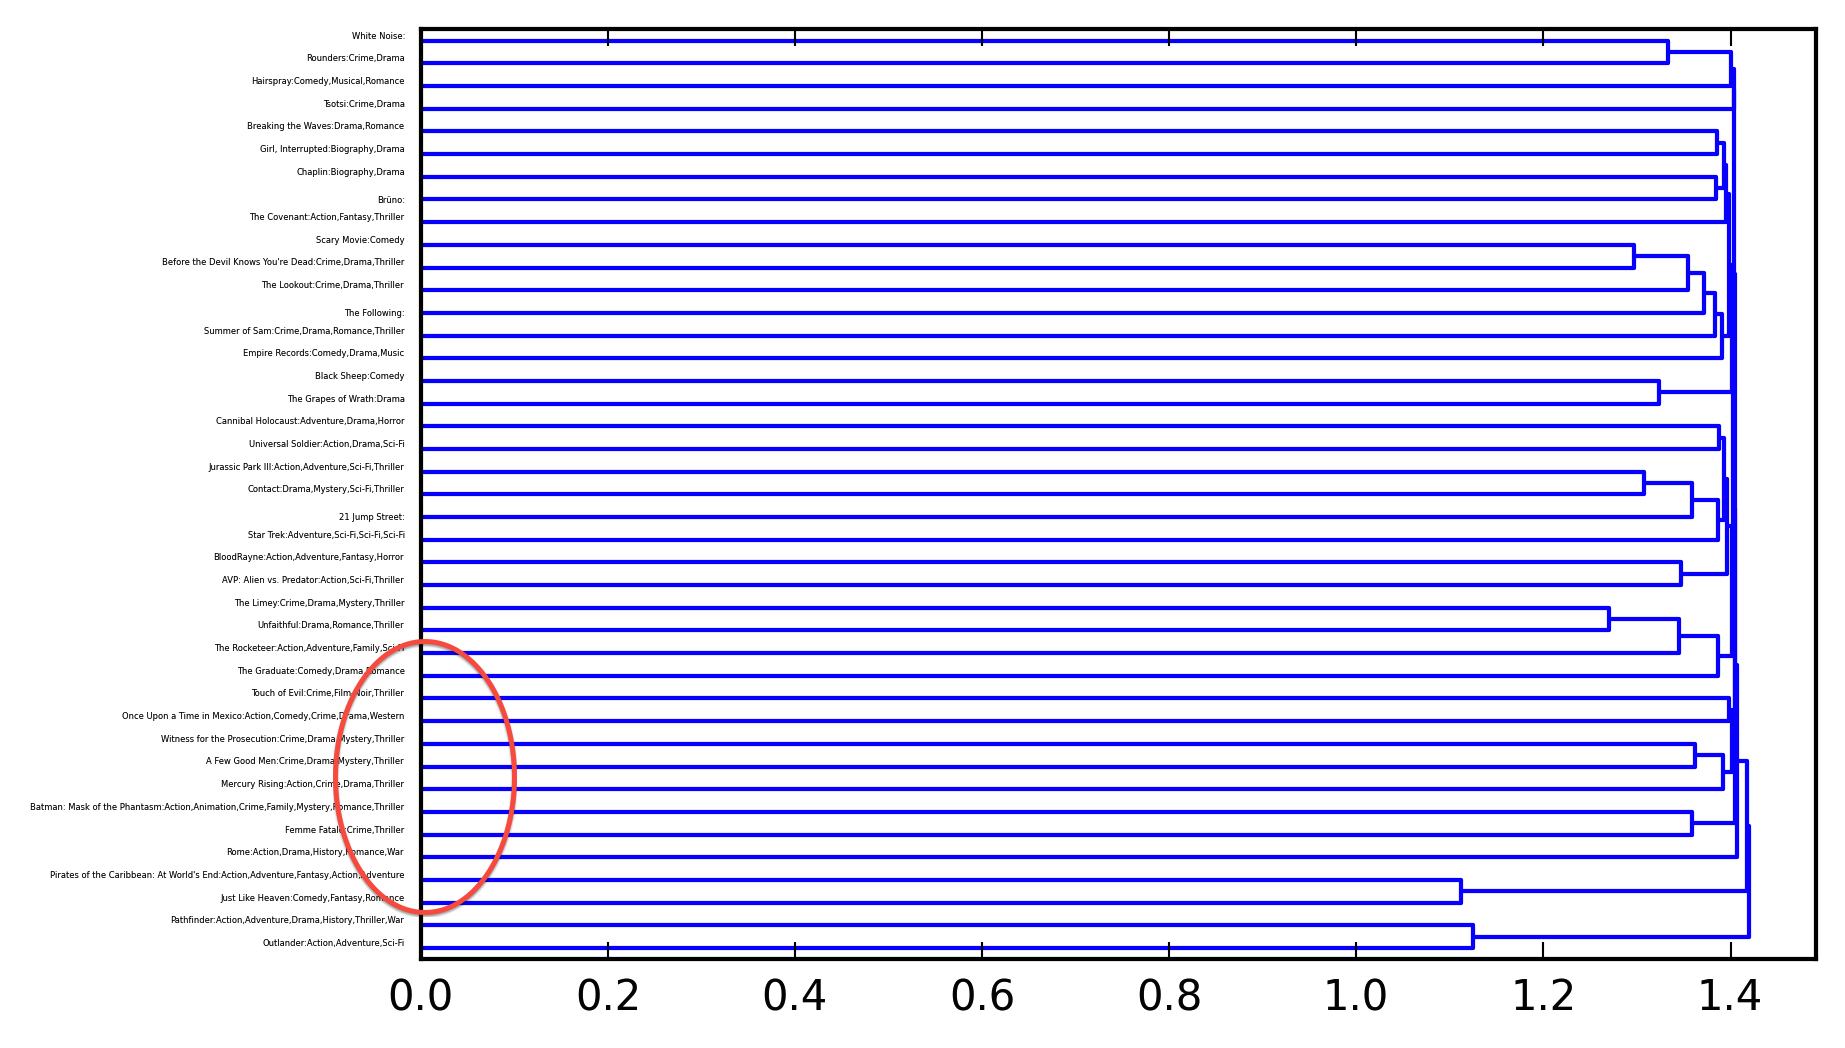
\includegraphics[width=0.6\linewidth]{img/clustering50_tf_idf.png}
	  \caption{Dendogram du hierachical clustering}
	  \label{hierarchical}
	\end{figure}
	
	En faisan un zoom sur limage (figure \ref{zoom}) on peut voire quel film a été groupé et on peut voire sa catégorie. Dans l'image ci-dessous on peut voir comme le film de la même catégorie a été groupé ensemble.
		\begin{figure}[h]
		  \centering
		    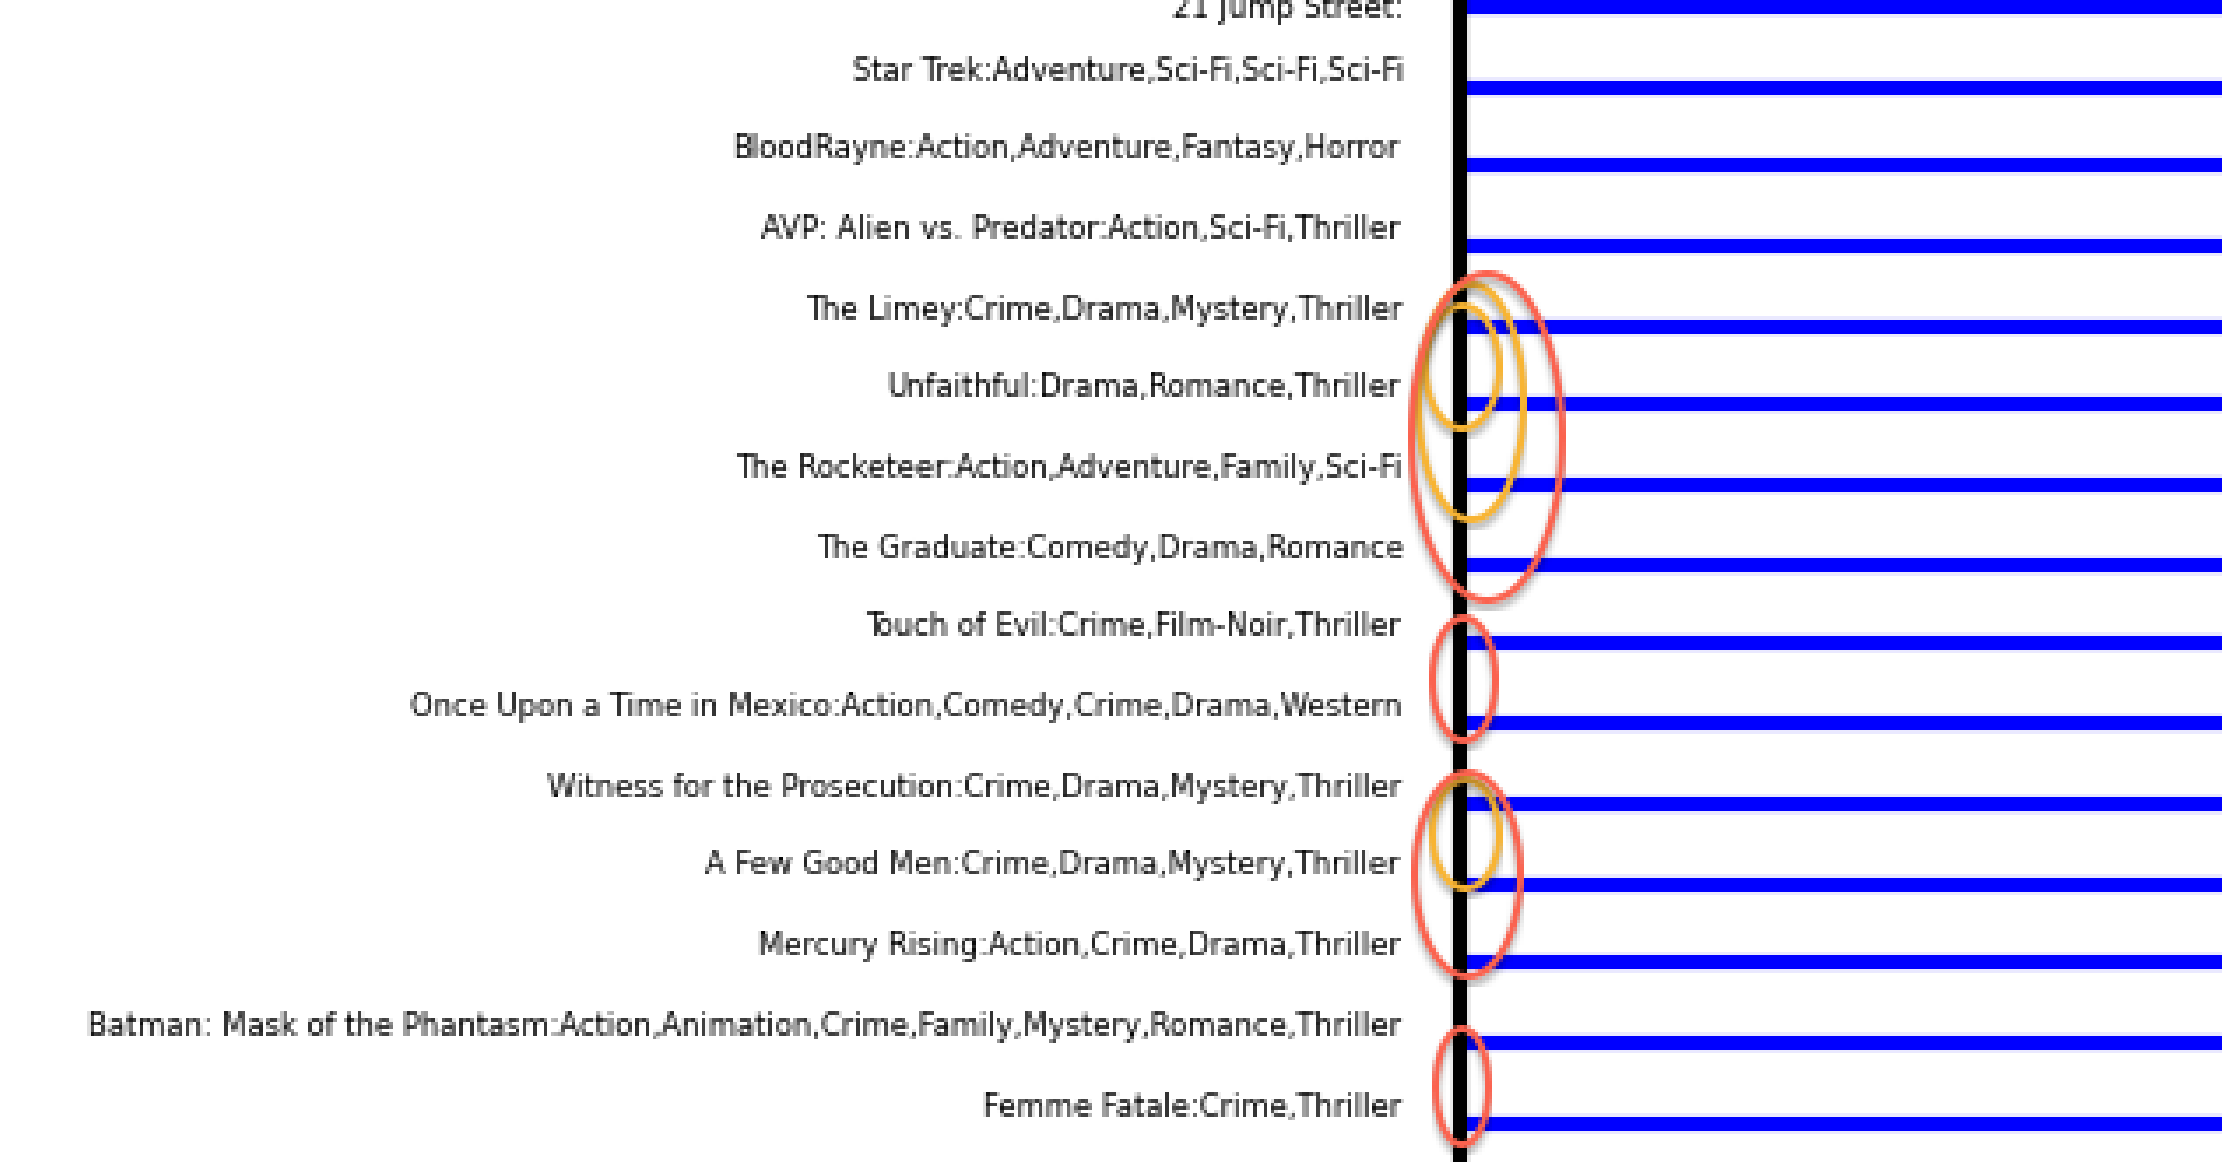
\includegraphics[width=1\linewidth]{img/zoom.png}
		  \caption{Dendogram du hierachical clustering, zoom}
		  \label{zoom}
		\end{figure}
		\newpage
	%Pour les films sans catégorie on peut cette fois les imaginer en regardant le groupement que l'algorithme a fait. Pour le film "Bruno" (figure \ref{bruno}) on peut en ne déduire que c'est similaire à "Chaplin" et qui aura une catégorie similaire a "Biography, Drama" ou peut-être il's ont simplement la description du film similaire. Peut-être aussi de ce deux films sont définissent une nouvelle catégorie. En regardant sur IMDB et en recherchant sur Wikipedia on peut voire qu’effectivement le film Bruno est un comédie drôle qui parle du personnage Bruno. On peut donc confirmer qui appartiens aussi à la catégorie "Biographie".
	Pour les films sans catégorie on peut cette fois les imaginer en regardant le groupement que l'algorithme a fait. Pour le film "White noise" (figure \ref{whitenoise}) on peut en ne déduire que c'est similaire à "Rounders" et qui aura une catégorie similaire a "Crime, Drama" ou peut-être il's ont simplement la description du film similaire. Peut-être aussi de ce deux films sont définissent une nouvelle catégorie. En regardant sur IMDB et en recherchant sur Wikipedia on peut voire effectivement le film "White noise" est dans les catégories "Drama, Mystery" c'est qui c'est donc vraisemblable avec notre résultats.
		
	 
		\begin{figure}[h]
			  \centering
			    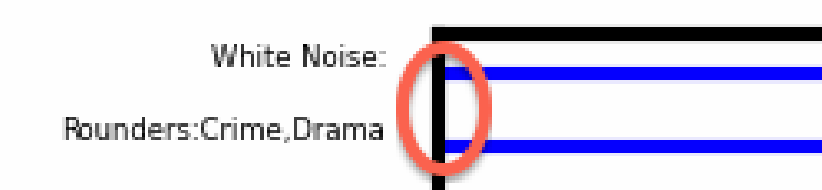
\includegraphics[width=0.6\linewidth]{img/whitenoise.png}
			  \caption{Dendogram du hierachical clustering, zoom}
			  \label{whitenoise}
			\end{figure}
	
	\section{Map de kohonen}
	Une fois avoir vu que l'algorithme est capable de reconnaitre les films avec une description similaire on peut utiliser un algorithme plus avancé pour avoir en sortie une map des films placés dans une région de la map. Les couleurs de la map représentent la distance entre chaque film. Rouge indique que la distance est grande et Bleut indique le contraire.
	
	La figure \ref{map1} montre un exemple d'un map généré avec 100 films.
	
	On peut voir depuis l'image
	\begin{figure}[h]
		\centering
		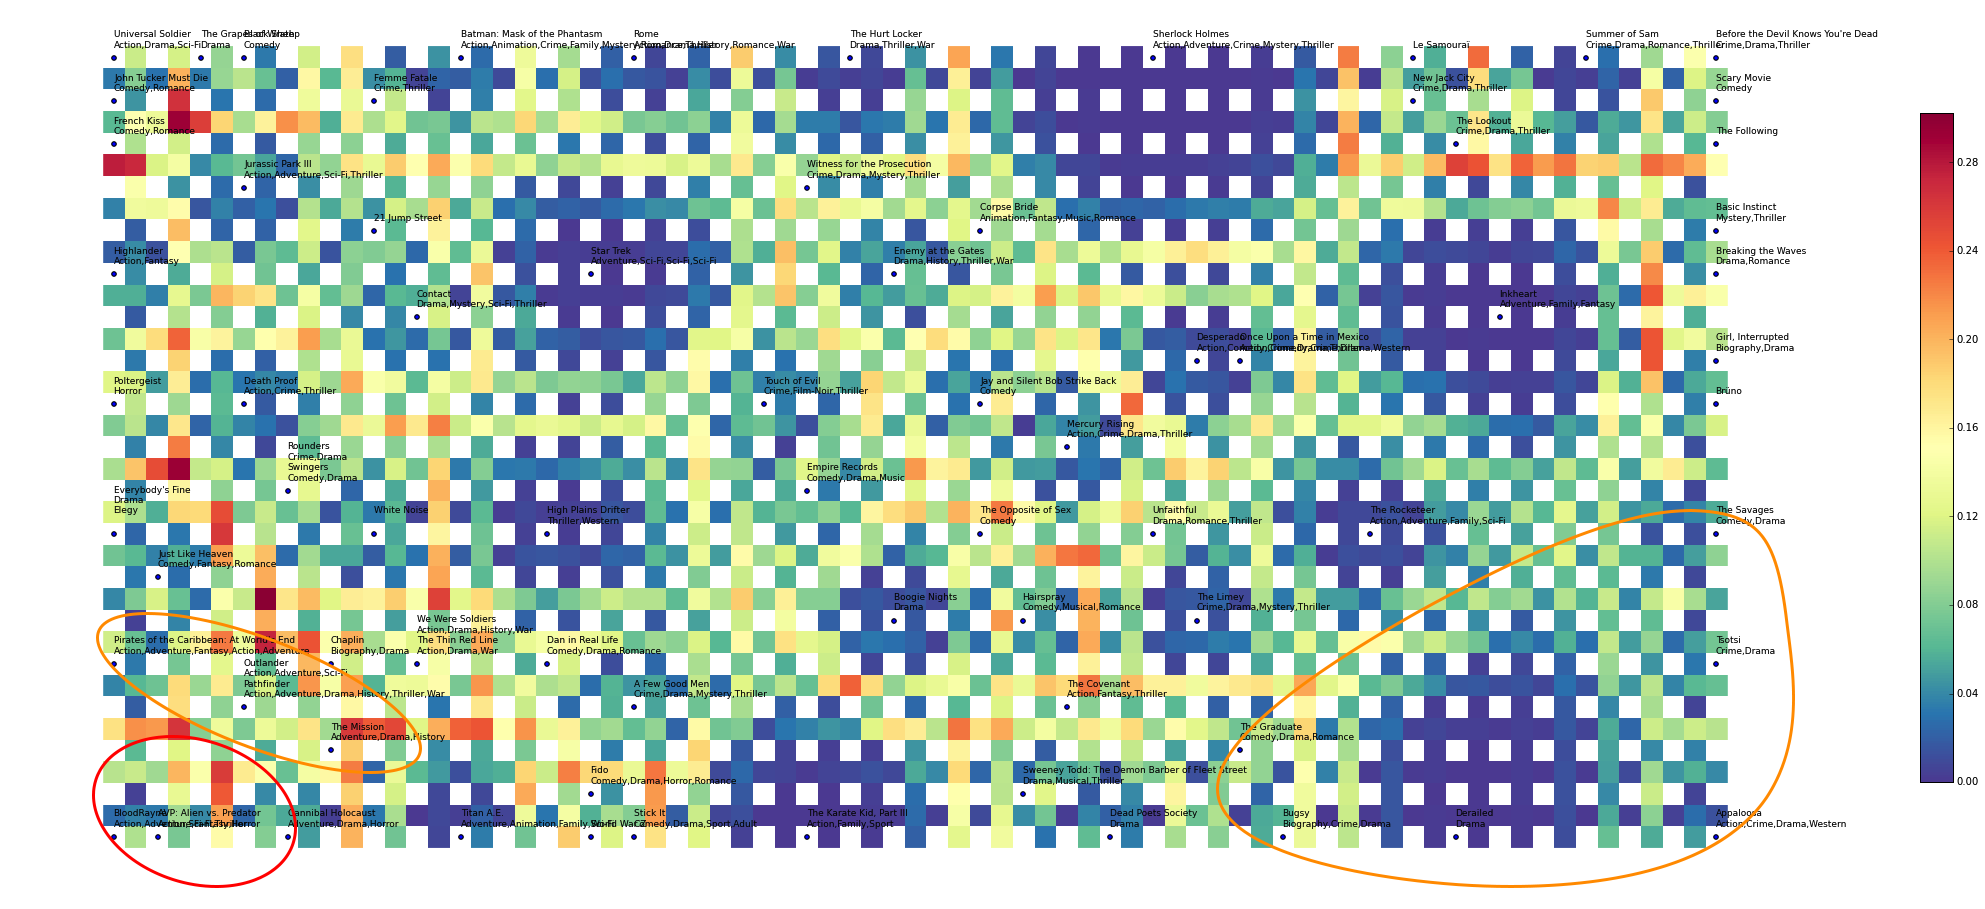
\includegraphics[width=1\linewidth]{img/map-cluster.png}
		\caption{Map de Kohonen avec 100 films}
		\label{map1}
	\end{figure}
	
	On peut voire depuis les couleurs de l'image qui il a de zones délimitées par de rouge, comme l'angle en bas à gauche et de zones délimitées par de vert ou jeune. La division en rouge indique que la division est beaucoup plus forte que celle jeune. Si on agrandit l'image on pourra voir le groupe des films similaire que la map de Kohon a créé.
	Dans l'image \ref{map1zoom2} agrandie on put voire que dans l'angle en bas à gauche on a de groupe délimité par de zones. On peut voire que l'algorithme mis dans l'angle en bas (cercle rouge) les "Bloody Rayan et Alient vs Predator" et on peut aussi voie que la catégorie donnée par IMDB est la même par le deux. On peut en déduire que la description de ce deux est effectivement similaire.
	
	Dans l'ellipse orange on peut voie un outre groupe résultant depuis la map de Kohonen qui met ensemble le filme d'action, d'aventure et "Drama".
	\begin{figure}[h]
		\centering
		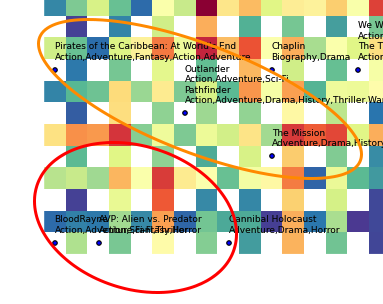
\includegraphics[width=0.5\linewidth]{img/map1zoom2.png}
		\caption{Map de Kohonen avec le zoom de l'angle en bas à gauche}
		\label{map1zoom2}
	\end{figure}
	\newpage
	Dans l'outre coté de l'image(figure \ref{map1zoom2} ) on peut voire une outre groupe des films. O voit que cette fois on regroupe les films avec les categories "Crime , Drama, Comedy, Biography". Même si les categorie sont legerement differentes on doit pense que la reconnessance est fait sur la description du film et pas sur d'outre parametre plus a haut niveau.
		
	\begin{figure}[h]
		\centering
		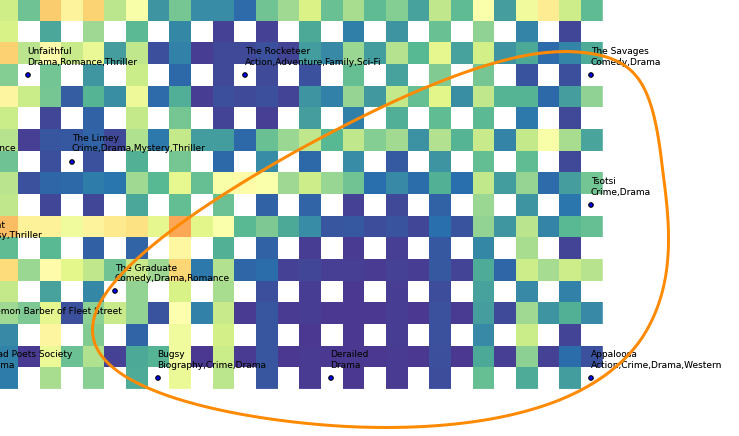
\includegraphics[width=0.6\linewidth]{img/map1zoom3.png}
		\caption{Map de Kohonen avec le zoom de l'angle en bas à droite}
		\label{map1zoom2}
	\end{figure}
	

 
 
 

